\chapter{Background on Probability and Statistics}\label{ch:statistics}
This chapter will discuss some statistical concepts that will be used to understand and build up the ideas behind the methodology of this paper, which is presented in the next chapter. With that said, the discussions are organized as follows: Section \ref{sec:descriptive_stat_method} will present the concept of Descriptive Statistics; Section \ref{sec:probability_method} will discuss the Probability Theory; and, Section \ref{sec:stat_graphs_method} will discuss the Statistical graphs or plots.

Further, the topics discussed here may be self-explanatory for Statisticians, ML researchers or those with Mathematical background. However, for the benefit of readers coming from humanities background, the paper will present the methodology as follows: mathematical formulas are formalized for purpose of brevity through Definition, Proposition, and Corollary, but immediate to these are explanations or examples aimed to be simple enough for non-statistician readers. As a guide, statisticians or ML researchers can simply read the Definition, Proposition, and/or Corollary. Whereas for humanities readers, the reading shouldn't not stress too much on the said mathematical formalities, and instead proceed to the discussions or examples immediate to it to aid with the understanding.
\section{Descriptive Statistics}\label{sec:descriptive_stat_method}
Among the basic statistical methodologies for summarizing information or data is what is known as Descriptive Statistics. From the name itself, these statistics are meant to convey simple descriptions of the data. For example, \textit{mean} and \textit{variance} are common statistics used for describing the data. The formulas for these statistics are given in the following definitions:
\begin{defn}[Mean]\label{defn:mean}
Let $x_i, i\in\{1,\cdots,n\}$ where $n\in\mathbb{N}$, then the \textit{mean} of $x_i$s is defined as follows:
\begin{equation}
    \bar{x} = \sum_{i=1}^n x_i, \qquad\text{where}\;x_i \in\mathbb{R}.
\end{equation}
\end{defn}
\begin{defn}[Variance]
    Let $x_i, i\in\{1,\cdots,n\}$ where $n\in\mathbb{N}$ and let $\bar{x}$ be the mean defined in Defn. \ref{defn:mean} then the \textit{variance} of $x_i$s is defined as follows:
    \begin{equation}
        \mathbb{V}\text{ar}(x) = \frac{1}{n-1}\sum_{i=1}^n (x_i-\bar{x})^2, \qquad\text{where}\;x_i \in\mathbb{R}.
    \end{equation}    
\end{defn}
\begin{defn}[Standard Deviation]
Let $\sigma^2$ be the variance, then the standard deviation, denoted by $\sigma$, is defined as $\sigma:=\sqrt{\sigma^2}$, that is, square root of the variance.    
\end{defn}
The mean is simply the average of the data points, while the variance is a single number that measures or summarizes the distances of the data points from the mean. The variance therefore measures how spread or varied the data points are. In practice, however, standard deviation is more popular for measure of variability since it doesn't get big easily due to the square root operator. Standard deviation is also the preferred metric for this paper.
\section{Probability Theory}\label{sec:probability_method}
Statistics is built around the concept of Probability Theory. Hence, it is important to understand how this mathematical theory behind the statistical concepts work. Probability theory is a discipline in itself. It is a branch of mathematics that aims at studying realizations or observations from random phenomena. It does this by using algorithms and models (\textit{see} discussion in Chapter \ref{ch:introduction} for understanding the model). These probability models are mathematical formula design to characterize or describe the patterns of data points. The simplest form of these models is the univariate probability density functions. However, before discussing these models, the idea behind it should be build up from ground up so that humanities readers can appreciate it. To do this, the discussion will proceed with the concept of probability.
\begin{defn}[Probability]\label{defn:probability}
A probability is a mathematical concept that measures the likelihood or chance of some event to happen.
\end{defn}
Indeed, this idea of probability is well known or is easily understood by many. So that, the probability that someone will die is 1, meaning 100\%, since that's how natures and biology work. Further, the probability of selecting one \arb[trans]{'ayAt} \arb{'ayAt} from \arb[trans]{sUraT 'l-fAti.hati} \arb{sUraT 'l-fAti.hati} through a random draw is one out of seven, assuming each \arb[trans]{'ayAt} \arb{'ayAt} has equal chances of being drawn.

Now, to gradually formalize the concept into mathematics, the succeeding definitions will be discussed to build up the definition of a probability distribution.
\begin{defn}[Sample Space]
Let $\omega_1,\cdots,\omega_n, \forall n\in\mathbb{N}$ be the list of all possible outcomes of a random event or a phenomena, then the sample space, denoted by $\Omega$, is defined as the collection of all these possible outcomes including the empty set denoted by $\emptyset$.
\end{defn}
\begin{exmp}\label{ex:sample_space}
Consider the random phenomenon or event where someone randomly picks a verse from the Qur'\=an, what is the probability that it will be a Meccan \arb{makkiyyaT} or a Medinan \arb{madaniyyaT} verse?

The possible output for such random event is either Meccan or Medinan. Suppose, we let Meccan to be denoted by $\omega_1$ and Medinan to be denoted $\omega_2$, then the sample space, which is the collection of all possible output is denoted as follows:
\begin{equation}\label{ex_eq:sample_space}
    \Omega:=\{\text{\arb{makkiyyaT}},\text{\arb{madaniyyaT}}\}=\{\text{Meccan}, \text{Medinan}\}=\{\omega_1,\omega_2\}
\end{equation}
It should be understood that $\emptyset$ is also included in $\Omega$, but is not written for brevity.

\end{exmp}
\begin{defn}[Event]
Let $\Omega=\{\omega_1,\cdots,\omega_n\}, \forall n\in\mathbb{N}$, be the sample space, then an event, denoted here as $\mathscr{A}$, is defined as the subset of the sample space, i.e., $\mathscr{A}\subseteq{\Omega}$.
\end{defn}
\begin{exmp}
From Ex. \ref{ex:sample_space}, consider drawing two samples from the Qur'an, what is the sample space and give an example of a possible event?\\
\textit{Solution:} The sample space is given below:
\begin{align}
    \Omega=&\{(\text{\arb{makkiyyaT}},\text{\arb{makkiyyaT}}),(\text{\arb{makkiyyaT}},\text{\arb{madaniyyaT}}), (\text{\arb{madaniyyaT}}, \text{\arb{makkiyyaT}}), (\text{\arb{madaniyyaT}}, \text{\arb{madaniyyaT}})\}\nonumber\\
    =&\{(\text{Meccan},\text{Meccan}),(\text{Meccan},\text{Medinan}), \\
    &\;\;(\text{Medinan},\text{Meccan}), (\text{Medinan},\text{Medinan})\}\\
    =&\{(\omega_1,\omega_1),(\omega_1,\omega_2),(\omega_2,\omega_1),(\omega_2,\omega_2)\}
\end{align}
So that, if $\mathscr{A}$ is the event of drawing two \arb[trans]{'ayAt} \arb{'ayAt} from the Qur'\=an, then a possible event is given by 
\begin{equation}
    \mathscr{A}:=\{\text{\arb{madaniyyaT}}, \text{\arb{makkiyyaT}}\}=\{\text{Medinan}, \text{Meccan}\}=\{\omega_2,\omega_1\}
\end{equation}
Therefore, $\mathscr{A}\subseteq\Omega$, read as $\mathscr{A}$ is a subset of $\Omega$.
\end{exmp}
Now, going back to the discussion on the concept of probability above and reflect on the example given, that the probability that someone will die is 1; and that the probability of selecting one \arb[trans]{'ayAt} \arb{'ayAt} from \arb[trans]{sUraT 'l-fAti.hati} \arb{sUraT 'l-fAti.hati} through a random draw is one out of seven. It therefore begs the following questions: how does one solve this? Like how does it translate into a formal mathematical computation?

Indeed, to appreciate the motivation of the succeeding definitions, it is important to devise a logical approach to computing probability mathematically, and this should explain why the following definitions are defined the way they are.

Probability as already defined in Defn. \ref{defn:probability} is a measure, which will be formalized in Defn. \ref{defn:probability_measure}. Indeed, this is analogues to measuring an object's size using a tape measure. So, when someone attempts to measure an object's size, there are conditions for the space of the object to be measurable. The first expectation is that, the space or area can be measured in several ways. Either measuring it as a whole, or measuring it piece by piece from its partitions. Now, measuring it as a whole using tape measure should be straightforward. However, measuring it by pieces can have several cases, and all of these should end up to the same measuring. These cases accounts for the fact that when dealing with pieces of the surface one can start with different sizes of the pieces to be measured. So that, all the collections of all these possible configurations of pieces are mathematically called $\sigma$-algebra, and this collection should include the following:
\begin{enumerate}
    \item The 0 size piece, that is, the object's measurement should start at 0;
    \item The remainings of the pieces given the pieces already measured;
    \item The union of all the pieces.
\end{enumerate}
The above explanation for the $\sigma$-algebra is condensed in to the following mathematical definition:
\begin{defn}[$\sigma$-algebra]\label{defn:sigma_algebra}
Let $\Omega:=\{\omega_1,\cdots,\omega_n\}, \forall n\in\mathbb{N}$, then the collections of all disjoint partitions, which are the events, are defined as the $\sigma$-algebra or $\sigma$-field, denoted here as $\mathfrak{F}$, and should satisfy the following conditions:
\begin{enumerate}
    \item The empty set $\emptyset\in\mathfrak{F}$
    \item If $\mathscr{A}\in\mathfrak{F}$, then the complement $\Omega\backslash\mathscr{A}$ is also an element of $\mathfrak{F}$
    \item If $\mathscr{A}_1,\mathscr{A}_2,\cdots$ is a countable sequence of sets in \mathscr{A}, then the $\bigcup_{i=1}^{\infty}\mathscr{A}_i$ is also an element of $\mathfrak{F}$
\end{enumerate}
\end{defn}
\begin{exmp}
Given the sample space $\Omega:=\{\text{Meccan},\text{Medinan}\}$, the $\sigma$-algebra is
\begin{align}
    \mathfrak{F}=&\{\text{Meccan},\text{Medinan},(\text{Meccan},\text{Medinan}),\nonumber\\
    &\;\;(\text{Meccan},\text{Meccan}), (\text{Medinan},\text{Meccan}),\nonumber\\
    &\;\;(\text{Medinan},\text{Medinan}),\emptyset\}
\end{align}

\end{exmp}
\begin{defn}[Probability Measure]\label{defn:probability_measure}
Let $\Omega$ be the \textit{sample space}, $\mathfrak{F}$ be the $\sigma$-algebra, $ p$ be the probability measure, then the probability of a set $\mathscr{A}, \mathscr{A}\in\mathfrak{F}$, on the probability space $(\Omega,\mathfrak{F}, p)$, denoted by $ p(\mathscr{A})$, satisfies the following properties:
\begin{enumerate}
    \item Non-negativity: For any set $\mathscr{A},  p(\mathscr{A})\geq 0$
    \item Normalization: $ p(\Omega)=1$
    \item Countable additivity: For any sequence of disjoint sets $\mathscr{A}_1,\mathscr{A}_2,\cdots$ in $\mathfrak{F}$, such that the union $\bigcup_{\forall i \in\mathbb{N}}\mathscr{A}_i$ is also in $\mathfrak{F}$, we have: $ p\left(\displaystyle\bigcup_{\forall i\in\mathbb{N}}\mathscr{A}_i\right)=\displaystyle\sum_{\forall \in\mathbb{N}} p(\mathscr{A}_i)$
\end{enumerate}

\end{defn}

Basically, the idea of Defn. \ref{defn:probability_measure} is to define the concept of "measure" in general sense, although above is a special measure called probability measure. As before, one can think of this probability measure like a tape measure in simple sense. This tape measure has some properties that should be expected for a measurement tool. The first property or condition is that the probability measure has to be positive. Indeed, if we use any tape measure for measuring length, never will someone get a negative measure like -2cm length. It always has to be positive. Further, the second condition to expect is that for this type of tape measure called probability measure, the total measure of all objects available in the given space should be equal to 1. That is, the total is normalized to 1. Think of this like 100\% coverage if we measure all of the objects. Lastly, for any object, this tape measure should be able to measure the object through partitions, such that the measure of the union of these partitions is equal to the sum of the measure of each partition. All of these conditions are logical criteria for a general idea of "measure," although the normalization part above is unique for probability measure. Note that, the concept of proability measure here should not be confined to measuring length as in the analogy, it should generalize to measuring volume and complex objects in general.
\begin{defn}[Random Variable]
Let $\Omega$ be the sample space, and $\mathbb{R}$ be the set of all real numbers, then a random variable $X$ is a function defined as $X:\Omega\rightarrow\mathbb{R}$.
\end{defn}
\begin{exmp}\label{ex:ayah_prob}
Consider the example of drawing a random verse or \arb[trans]{'ayAt} \arb{'ayAt} again, what is the probability that it will be an \arb[trans]{'ayAt} \arb{'ayAt} from \textit{s\=urah l-baqara}'s \arb[trans]{'ayAt} \arb{A"'yaTu sUraT 'l-baqaraT} or the Chapter of Cow?

The answer to this is 4.59\% probability, this is because there are 286 \arb[trans]{'ayAt} \arb{'ayAt} and there are 6236 verses in the Qur'\=an, so that the probability is $\frac{286}{6236}=0.04586$. The assumption here is that all of the \arb[trans]{'ayAt} \arb{'ayAt} in the Qur'\=an have equal chances of being picked up or drawn.

\end{exmp}
\begin{exmp}\label{ex:binom_manual}
To apply the concept so far, consider again Ex. \ref{ex:ayah_prob}, what is the probability of getting 5 \textit{s\=urah l-baqara}'s \arb[trans]{'ayAt} \arb{A"'yaTu sUraT 'l-baqaraT} if we randomly pick 20 \arb[trans]{'ayAt} \arb{'ayAt} in total from the Qur'\=an?\\
\textit{Solution.} The following are given:
\begin{itemize}
    \item $n=20$ independent trials of drawing $x=5$ \arb{'ayAt} from the Qur'\=an
    \item Each trial has two possible outcomes: \arb[trans]{na`am} \arb{na`am} meaning Yes or \arb[trans]{lA} \arb{lA} meaning No. That is, if the \arb[trans]{'ayAt} \arb{'ayAt}  is from the \textit{s\=urah l-baqara} \arb{sUraT 'l-baqaraT} then its \arb{na`am}, otherwise \arb{lA}.
\end{itemize}
Now, the sample space consists of all possible sequences of 20 \arb{na`am} and \arb{lA}. That is,
\begin{align}
    \Omega=\{&
        (\text{\arb{lA}},\text{\arb{na`am}},\text{\arb{lA}},\cdots,\text{\arb{na`am}}),\\
        &(\text{\arb{lA}},\text{\arb{na`am}},\text{\arb{lA}},\cdots,\text{\arb{lA}}),\\
        &\qquad\qquad\vdots\\
        &(\text{\arb{lA}},\text{\arb{lA}},\text{\arb{lA}},\cdots,\text{\arb{lA}})\}.
\end{align}
In total, there are $20^2=400$ possible samples in the sample space $\Omega$. Further, from Ex. \ref{ex:ayah_prob}, the probability of getting a \textit{s\=urah l-baqara}'s \arb[trans]{'ayAt} \arb{A"'yaTu sUraT 'l-baqaraT} is 0.0459 or 4.59\%. Therefore, if $X$ is the random variable of an event of drawing an \arb[trans]{'ayAt} from the Qur'\=an, if we assign \arb{lA}  and \arb{na`am} as either 0 or 1, respectively, then this would imply that mathematically $ p(X=1)=0.0459$. In addition, the probability of getting an \arb[trans]{'ayAt} \arb{'ayAt} from other \textit{s\=urah} \arb{sUraT} would be

\begin{equation}    
 p(X=0)=1- p(X=1)=1-0.0459=0.9541.
\end{equation}

Further, let $Z$ be the random variable for the event of getting $n$ \arb{na`am} from 20 trials, then the problem is now equivalent to finding the number of ways to choose $n$ possible positions out of 20 in the collection or set. This can be solved using the \textit{combination} formula as shown below:
\begin{align}
    n \choose x &= \frac{n!}{r!(n-r)!}\Rightarrow{20 \choose 5} = \frac{20!}{5!(20-5)!}=15,504. 
\end{align}
That is, there are 15,504 possible cases of 5 positions' configuration for \arb{na`am} in a 20 trial. Moreover, in each of these samples 5 has a probability of $ p(X=1)=0.0459$, while the remaining 15 has a probability of $ p(X=0)=0.9541$. So that,
\begin{align}
     p(Z=5)&=184,756\times p(X=1)^{5}\times p(X=0)^{20-5}\nonumber\\
    &=15,504\times0.0459^{5}\times0.9541^{20-5}\nonumber\\
    &=0.0016.
\end{align}
Hence, there is a 0.16\% probability of getting 5 \textit{s\=urah l-baqara}'s \arb[trans]{'ayAt} \arb{A"'yaTu sUraT 'l-baqaraT} when randomly drawing 20 \arb{'ayAt} from the Qur'\=an.

\end{exmp}
Note that Ex. \ref{ex:binom_manual} can be solved using a known formula in probability called \textit{Binomial} mass function, which is a model that can be used to describe the event of getting 5 \textit{s\=urah l-baqara}'s \arb[trans]{'ayAt} \arb{A"'yaTu sUraT 'l-baqaraT} on a 20 random samples of Qur'\=an's \arb{'ayAt}. The {Binomial} mass function is specifically a probability mass/density function model. The following section will discuss the Statistical Graphs, which will cover the concept of frequency distribution, the one modeled or characterized by the probability mass/density function.
\section{Statistical Charts}\label{sec:stat_graphs_method}
Charts or plots or graphs are data visualization tools that are useful for exploratory data analysis apart from the Descriptive Statistics discussed above. It supplements the Descriptive Statistics findings through shapes visualized in the graphs. Among the popular statistical graphs is the bar graph. An example of this is given in Figure \ref{fig:ayah_word_count}. Other graphs used are the box plots and the density plots which is also in Figure \ref{fig:ayah_word_count}
\subsection{Box, Density, and Histogram Plots}
While most statistical plots are easy to understand like bar graphs and scatter plots, others like Box, Density, and Histogram plots may not be easy to comprehend for someone with no Statistical background. This section will discuss how it is interpreted. Let's use Figure \ref{fig:ayah_word_count}, Figure \ref{fig:ayah_word_count_with_desc} for easy reference in this section.
\begin{figure}[!b]
    \centering
    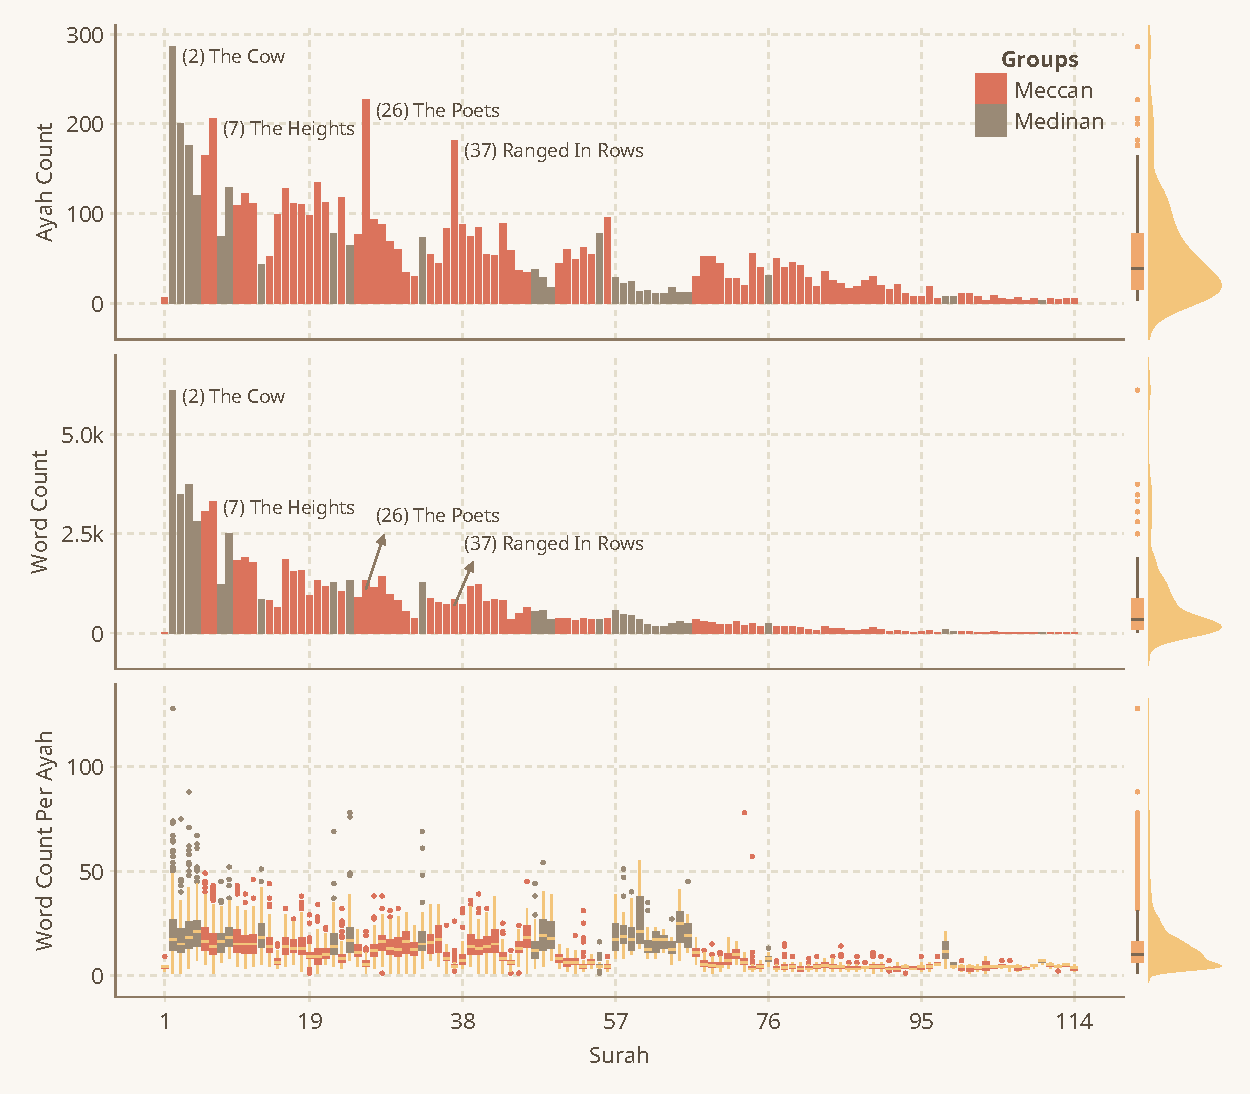
\includegraphics[width=\textwidth]{img/plot1.pdf}
    \caption{Statistics of the words and \arb[trans]{ayAt} \arb{ayAt} (verses) of the Qur'\=an}
    \label{fig:ayah_word_count_with_desc}
\end{figure}

As shown in Figure \ref{fig:ayah_word_count_with_desc}, both the Box and Density plots are tied to each other. This is indeed the case because both are describing the same information but presented in different style of visualization. In fact, Histogram is also used to describe the same information as the Box and Density, and the three are therefore related. So much so, that the three can be put into one graph. As to how to interpret these, readers are referred to for further details \textcolor{red}{[to add reference]}.
\begin{exmp}[Frequency Distribution]\label{ex:frequency_distribution}
Consider again the task of drawing an \arb[trans]{'ayAt} \arb{'ayAt} from the Qur'\=an, suppose the \arb[trans]{'ayAt} \arb{'ayAt} are separated into \arb{makkiyyaT} Meccan and \arb{madaniyyaT} Medinan, what is the probability of getting at most 10 \arb[trans]{kalimAt} \arb{kalimAt} or words in a sampled \arb[trans]{'ayAt} \arb{'ayAt} from \arb{makkiyyaT} Meccan \textit{surah}s \arb{sUr}?\\
\textit{Solution:} To answer this, Figure \ref{fig:meccan_medinan_word_count_per_ayah} shows the \textit{histograms} with the \textit{box plots} and the \textit{rainclouds} plots. The figure shows the frequency of the \arb[trans]{kalimAt} \arb{kalimAt} or words in a sampled \arb[trans]{'ayAt} \arb{'ayAt}. This frequency describes the distribution of the \arb[trans]{kalimAt} \arb{kalimAt}. To interpret this, the Medinan \arb{madaniyyaT} histogram shows that most of the \arb[trans]{'ayAt} \arb{'ayAt} have about 10 to 20 \arb[trans]{kalimAt} \arb{kalimAt} or words in total. This conclusion is based on the where the box of the box plot is located, which also corresponds to the area where the bars of the histogram are high, and also where most of the points or 'droplets' from the rainclouds plot are congested. With that said, \textit{historgram}, \textit{box plot}, and \textit{rainclouds} are related and are telling the same story from different perspectives. It should be noted that, the rainclouds plot is not a common visualization tool. 

Now, comparing the numbers from Medinan \arb{madaniyyaT} to the \arb[trans]{'AyAt 'l-makkiyyaTu} \arb{'AyAt 'l-makkiyyaTu}, there are about 5 to 15 \arb[trans]{kalimAt} \arb{kalimAt} to expect per \arb[trans]{'ayAt} \arb{'ayAt} based on Figure \ref{fig:meccan_medinan_word_count_per_ayah}. 

\begin{figure}[!t]
    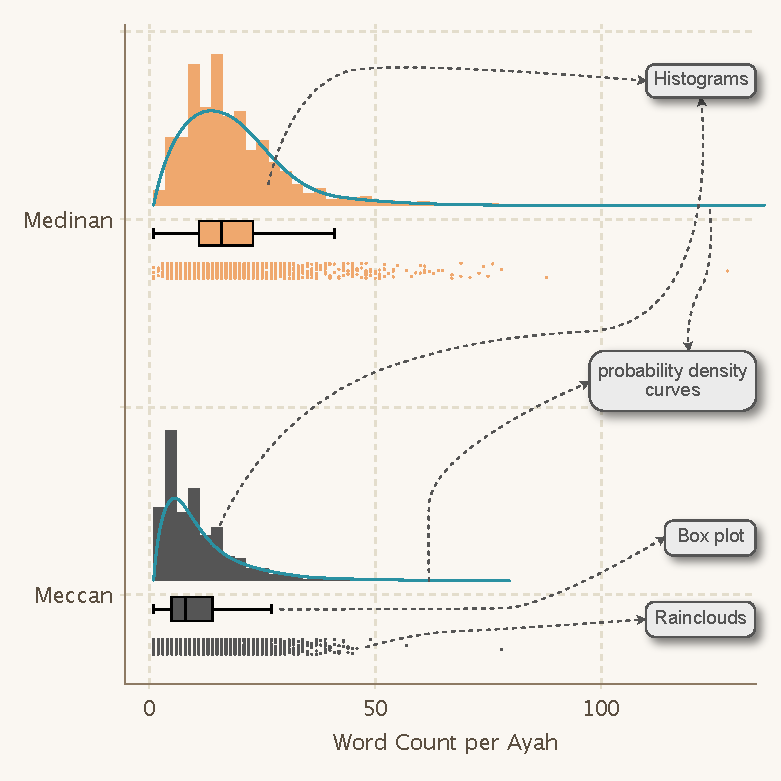
\includegraphics[width=\textwidth]{img/plot3.pdf}
    \caption{Probability density function plot of word count per \arb[trans]{'ayAt} \arb{'ayAt} by revelation location, in relation to its box plot and rainclouds.}
    \label{fig:meccan_medinan_word_count_per_ayah}
\end{figure}

The question has not been answered yet though, the above discussions only explains how to interpret the graphs in Figure \ref{fig:meccan_medinan_word_count_per_ayah}. So to answer the question, one simply needs to total the number of \arb[trans]{'AyAt} \arb{'AyAt} with at most 10 \arb[trans]{kalimAt} \arb{kalimAt} or words and divide this with the total number of \arb[trans]{'AyAt 'l-makkiyyaTu} \arb{'AyAt 'l-makkiyyaTu}. The answer is as follows, and this is part of the result of this paper: there are 4613 \arb[trans]{'AyAt 'l-makkiyyaTu} \arb{'AyAt 'l-makkiyyaTu}, and out of these is 2602 \arb[trans]{'AyAt 'l-makkiyyaTu} \arb{'AyAt 'l-makkiyyaTu} with at most 10 words. Therefore, the probability is $\frac{2602}{4613}=0.612$ or 61.2\% probability. Formally, if $X$ is the random variable of the event of observing at most 10 \arb[trans]{kalimAt} \arb{kalimAt} in a \arb[trans]{'AyAt 'l-makkiyyaTu} \arb{'AyAt 'l-makkiyyaTu}, then 
\begin{align}
     p(X\leq 10)=&\sum_{x=0}^{10} p(X=x)\label{ex_eq:prob_lesseq_10}\\
    =& p(X=0)+ p(X=1)+ p(X=2)+\cdots+ p(X=10)\label{ex_eq:freq_dist_prob1..10}\\
    =&0+\frac{24}{4613}+\frac{172}{4613}+\cdots+\frac{222}{4613}\label{ex_eq:freq_dist_probval1..10}\\
    =&\frac{2602}{4613}=0.612\label{ex_eq:prob_0612}
\end{align}

From Eq. \ref{ex_eq:freq_dist_prob1..10}, $ p(X=0)$ is the probability of observing zero \arb[trans]{kalimaT} \arb{kalimaT} in a \arb[trans]{'AyAt 'l-makkiyyaTu} \arb{'AyAt 'l-makkiyyaTu}, and $ p(X=1)$ is the probability of observing one \arb[trans]{kalimaT} \arb{kalimaT} in a \arb[trans]{'AyAt 'l-makkiyyaTu} \arb{'AyAt 'l-makkiyyaTu}, and so on. The numbers in Eq. \ref{ex_eq:freq_dist_probval1..10} are the number of \arb[trans]{'AyAt 'l-makkiyyaTu} \arb{'AyAt 'l-makkiyyaTu} having zero, one, two, to ten \arb[trans]{kalimAt} \arb{kalimAt}.

\end{exmp}
\section{Population and Sample}
Statistics is a branch of science that is concerned with understanding how the data behave based on a sample---a small set of the said data. It uses statistical methodologies to understand these behavior such as probability mass/density function, and use the findings from these tools on the sampled data as a conclusion for the population---the overall data.

Figure \ref{fig:pop_sample} illustrates the relation of population and sample data. A good example of this is the political surveys on the pulse of the nation on the candidates prior to election. Private entities like PulseAsia\footnote{\url{https://pulseasia.ph/}} and Social Weather Station\footnote{\url{https://www.sws.org.ph/swsmain/home/}} (SWS) do their survey by  sampling from the total population of the Philippines, hence the name survey.

The statistics computed from the surveys like the percentage of votes for particular political candidate are referred as estimates, this is because the computation was done in a sample of the population and not on the population itself. It is therefore important that for these estimates to be accurate representation of the nation's opinion, it has to be representative of the population. That is, the sample shouldn't be bias and leaning to the opinions of the few only and not of the whole nation.

The importance of the sample data as illustrated below follows from the fact that it saves time and cost since interviewing 2500 compared to 100,000 is better compromise for the estimated vote percentages. Further, since these samples requires to well represent the population, the computations of the statistics are estimated using statistical models, like probability mass/density functions, and other models like linear and nonlinears discussed in Section \ref{sec:stat_modeling}. The next example will illustrate the idea population and sample, and how probabilistic modeling can help in understanding insights and answering more questions.
\begin{figure}[t]
    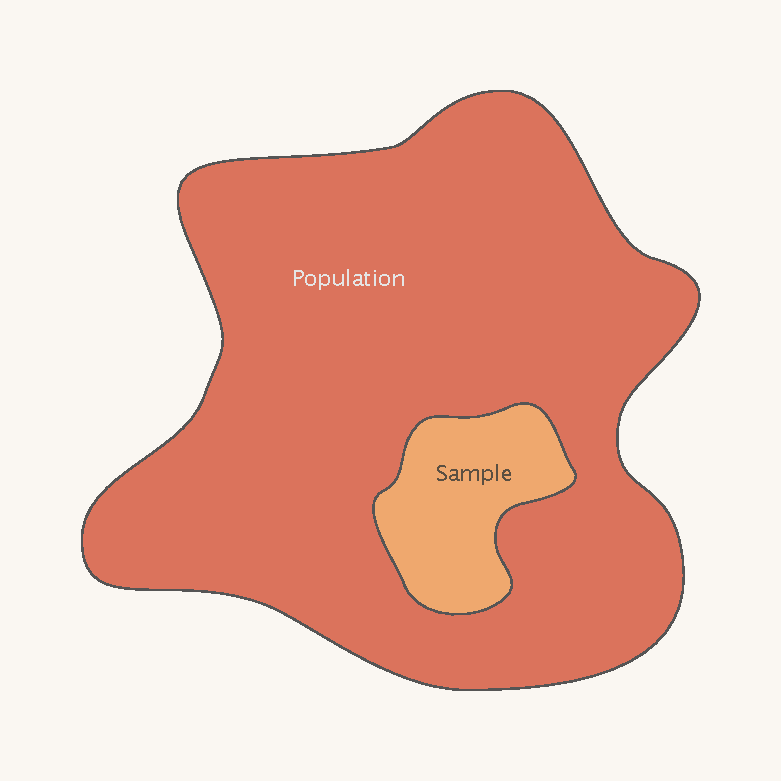
\includegraphics[width=\textwidth]{img/pop_sample.pdf}
    \caption{Population and sample illustration}
    \label{fig:pop_sample}
\end{figure}
\begin{exmp}\label{ex:population_sample_distribution_meccan_words}
Consider the task of sampling 250 \arb[trans]{'AyAt} \arb{'AyAt} from the population of \arb[trans]{'AyAt 'l-makkiyyaT}, describe the statistics of the population and the sample.\\
\textit{Solution:} In Statistics, there are several ways to sample from data, the simplest approach is through the use of \textit{uniform distribution}, that is, the sampling assumes that all data from the population are distributed equally, in the sense that all data points have equal chance of being selected. The other approach is through a \textit{weighted distribution}, where a probability is assigned to each of the data points in the population, so that, the selection will be biased to those with high probability. Figure \ref{fig:meccan_words_sampling} shows the graphs or plots of the population distribution of \arb[trans]{kalimAtu 'l-makkiyyaT} \arb{kalimAtu 'l-makkiyyaT}, which is presented as the top plot, this distribution of \arb{kalimAtu 'l-makkiyyaT} is the same one shown in the bottom plot of Figure \ref{fig:meccan_medinan_word_count_per_ayah}. 

To draw 100 samples from the said population, a simple random sampling without replacement (SRSWOR) is used for selecting or drawing samples. SRSWOR works by randomly selecting sample from the population and then setting it aside as the first sample. The resulting 100 samples are plotted in the bottom plot of Figure \ref{fig:meccan_words_sampling}.

As discussed above, the sample needs to be representative of the population. Figure \ref{fig:meccan_words_sampling} shows that the sampling distribution has more or less the same shape as the population. So that, the statistics are shown in Table \ref{tbl:meccan_words_pop_sample_stats}. From the said table, it can be seen that in terms of centrality, the both data are almost the same, for example the mean is 12.42 for the population and 10.64 for the sample. The reason why the mean in the population is much higher is due to the outlier in the population, which is seen in the extent of the tail of the Kernel Density Estimate in Figure \ref{fig:meccan_words_sampling}. In fact, this is seen in the Median in Table \ref{tbl:meccan_words_pop_sample_stats}, where  the estimate are almost the same. This is because the median is not affected by the outlier. However, the variance did suffer from the outlier in the population, with 50\% reduction in the sample variance, 54.15 to 48.96. The sample will less likely get the outlier as the sample since the outlier is only one observation from the 4163 total Meccan surahs.

The estimates got from the sample ideally are taken from a probabilistic model fitted into the sample data. This computation will be discussed in the next example.

\begin{table}
    \caption{Descriptive statistics of the population and sample data of \arb[trans]{kalimAtu 'l-makkiyyaT} \arb{kalimAtu 'l-makkiyyaT}}
    \label{tbl:meccan_words_pop_sample_stats}
    \begin{tabularx}{\textwidth}[!h]{XXXXl}
        \toprule
        Data&Mean&Median&Variance&Std. Deviation\\
        \midrule
        Population&10.28&8&54.15&7.36\\
        Sample&10.64&9&48.96&7.00\\
        \bottomrule
    \end{tabularx}
\end{table}
\begin{figure}[t]
    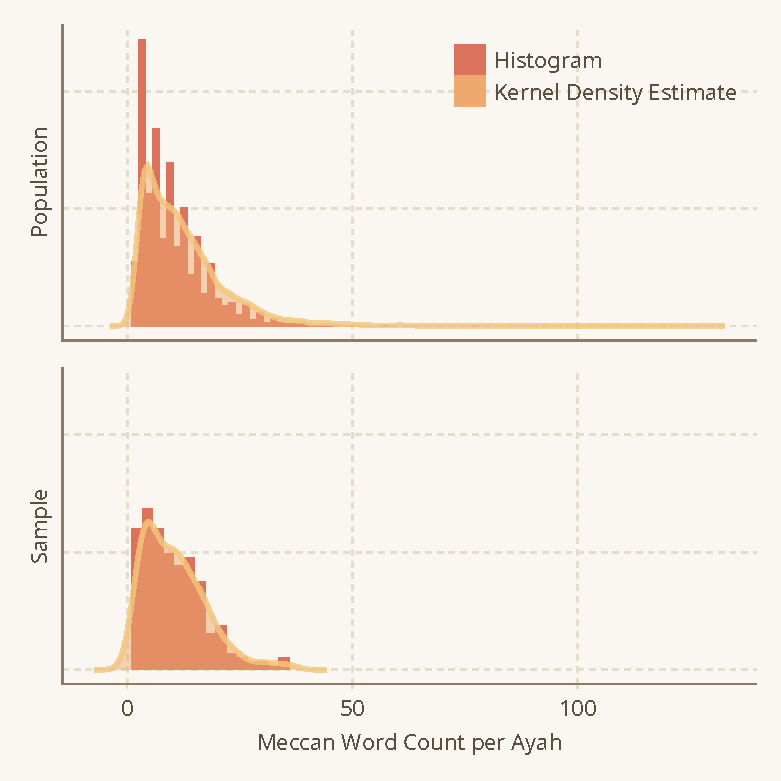
\includegraphics[width=\textwidth]{img/plot5.pdf}
    \caption{Population and sample distribution of Meccan }
    \label{fig:meccan_words_sampling}
\end{figure}

\end{exmp}
\begin{exmp}
Consider again Ex. \ref{ex:population_sample_distribution_meccan_words}, suppose the sample data is the only data available, how will you compute the probability of getting exactly 35 \arb[trans]{kalimAtu 'l-sUratu 'l-makkiyyaTu} \arb{kalimAtu 'l-sUratu 'l-makkiyyaTu}?\\
\textit{Solution:} To answer this question, one might approach this using the frequency distribution as in Ex. \ref{ex:frequency_distribution}. However, the use of frequency distribution from the said example is applicable since that deals with the population data, which is already the true probability, and there is no need to do some estimation. It is like try to get the average height of male Filipinos in the Philippines by doing census across the population, for such case, why would you do an estimate if you have all the census data of all heights of the Filipino, wouldn't it be easier to just do the average computation directly? This is the analogy for the frequency distribution used in Ex. \ref{ex:frequency_distribution}, that is, no need to do some estimation. However, for this problem, the assumption is that only the sample is available, that is, not all of the population is available. With that said, the best solution is to do some estimation. Now, doing an estimation is possible using the samples only, that is, using the idea of frequency distribution but this time applying it on the sample. This is becaus the sample was done using a random sampling, which more or less representative of the population. However, using this approach may possess a problem, let's see what that problem will likely be by forcing the approach in Ex. \ref{ex:frequency_distribution}, following the computation as in Eq. (\ref{ex_eq:prob_lesseq_10}) to Eq. (\ref{ex_eq:prob_0612}). 

Let $X$ again be the random variable of an event of observing 35 \arb[trans]{kalimAt} \arb{kalimAt}, this time from the sample, then
\begin{equation}\label{eq:probx_eq_35}
     p(X=35)=\begin{cases}
        \displaystyle\frac{0}{250}=0,&\text{if sample data}\\
        \displaystyle\frac{5}{4613}=0.0011,&\text{if population data}
    \end{cases}
\end{equation}
From the Eq. \ref{eq:probx_eq_35}, it shows that if we use the sample data for estimating the probability of observing 35 \arb{kalimAt}, then the answer above is 0, meaning by estimate there is a 0 chance of observing a 35 \arb{kalimAt} from a \arb[trans]{'AyAtu 'l-makkiyyaTu} \arb{'l-sUrAtu 'l-makkiyyaTu}. This conclusion is indeed misleading, since according to the population data, there are \arb[trans]{'AyAtu 'l-makkiyyaTu} \arb{'AyAtu 'l-makkiyyaTu} that has 35 \arb[trans]{kalimAt} \arb{kalimAt}. 

So, how to properly estimate this then? This is where the concept of probabilistic modeling comes in. For this problem, the data is count, and that the event of observing 10 \arb[trans]{kalimAtu 'l-sUratu 'l-makkiyyaTu} \arb{kalimAtu 'l-sUratu 'l-makkiyyaTu} in an \arb{'ayaT} is known to be best modeled by a Poisson distribution defined in Defn. \ref{defn:poisson_mass_function}. Ex. \ref{ex:poisson_distribution_sample} will discuss how to solve this. 
\end{exmp}
\section{Probability Distributions}
\begin{defn}[Poisson Mass Function]\label{defn:poisson_mass_function}
Let $X$ be a random variable and let $\lambda>0$ be a parameter, then if $x$ is the random value, then the \textit{Poisson} mass function is given by:
\begin{equation}
     p(X=x)=\frac{\lambda^x\exp(-\lambda)}{x!}
\end{equation}
\end{defn}
\begin{exmp}\label{ex:poisson_distribution_sample}
Consider again Ex. \ref{ex:population_sample_distribution_meccan_words}, the problem can be solved using the Poisson distribution.
\end{exmp}
\begin{defn}[Normal Density Function]
Let $Y$ be a random variable and let $\mu\in\mathbb{R}$ and $\sigma\in\mathbb{R}$ be the mean and variance parameters, if $y$ is the random value, then the \textit{Gaussian} or \textit{Normal} density function is given below:
\begin{equation}
     p(Y=y):=\frac{1}{\sqrt{2\pi\sigma^2}}\exp\left\{-\frac{(y-\mu)^2}{\sigma^2}\right\},\quad\text{where}\;-\infty<y<\infty
\end{equation}
\end{defn}
\begin{defn}[Dirichlet Density Function]
Let $\mathbf{Y}$ be a vector random variable with a random value $\mathbf{y}:=[y_1,\cdots,y_k]^{\text{T}}$ and let $\boldsymbol{\alpha}:=[\alpha_1,\cdots,\alpha_k]^{\text{T}}$ be the parameters, then the \textit{Dirichlet} density function is defined as
\begin{equation}
     p(\mathbf{X}=\mathbf{x};\boldsymbol{\alpha}):=\frac{1}{B(\boldsymbol{\alpha})}\prod_{i=1}^kx_i^{\alpha_i-1},
\end{equation}
where,
\begin{equation}
    B(\boldsymbol{\alpha}):=\frac{\displaystyle\prod_{i=1}^k\Gamma(\alpha_i)}{\Gamma\left(\sum_{i=1}^k\alpha_i\right)}
\end{equation}

\end{defn}
\begin{defn}[Multinomial Mass Function]
Let $\mathbf{X}$ be a vector random variable with a random value $\mathbf{x}:=[x_1,\cdots,x_k]^{\text{T}}$ such that $x_i\geq 0,\forall i \in[1,k]$, let $\boldsymbol{q}:=[q_1,\cdots,q_k]^{\text{T}}$ and $n$ be the parameters, the probability mass function of a Multinomial distribution is 
\begin{align}
    f(x_1,\cdots,x_k;n,q_1,\cdots,q_k):=& q(X_1=x_1\;\text{and}\;\cdots\;\text{and}\;X_k=x_k)\nonumber\\
    =&\begin{cases}
        \displaystyle\frac{n!}{x_1!\cdots x_k!}q_1^{x_1}\times\cdots\times q_k^{x_k},&\text{when}\;\sum_{i=1}^kx_i=n\\
        0&\text{otherwise},
    \end{cases}
\end{align}
\end{defn}

\section{Frequentist Estimation}\label{sec:stat_modeling}
Probability distributions are fundamental models that can be used to describe some characteristics of the data. However, combinations of variables, and accounting dynamics of the observations can lead into other types of models as well. In general, a statistical model can be written using the following formula:
\begin{equation}
    y=f(x|\mathbf{\Theta})+\varepsilon,
\end{equation}
where $y\sim p(\cdot)$ and $\varepsilon\sim p(\cdot)$.

There are two main ways to estimating the parameters $\boldsymbol{\Theta}$, and that is either through Frequentist or Bayesian approach.
\subsection{Maximum Likelihood Estimation}
Maximum likelihood estimation (MLE) is a fundamental concept in statistics that provides a method for estimating the parameters of a statistical model based on the observed data. The basic idea behind MLE is to find the parameter values that make the observed data most likely or probable under the assumed statistical model. The concept of MLE can be explained as follows:

Suppose we have a random sample of observations $X := \{x_1, x_2, ..., x_n\}$ from a probability distribution $f(x | \theta)$, where $\theta$ represents the unknown parameter(s) of the distribution. The likelihood function, denoted as $\mathcal{L}(\theta | X)$, is the joint probability density (or probability mass function for discrete distributions) of the observed data $X$, treated as a function of the parameter(s) $\theta$.
\begin{equation}
    \mathcal{L}(\theta | X) = f(x_1 | \theta) \times f(x_2 | \theta) \times\cdots\times f(x_n | \theta)    
\end{equation}

The maximum likelihood estimate (MLE) of $\theta$, denoted as $\hat{\theta}$, is the value of $\theta$ that maximizes the likelihood function $\mathcal{L}(\theta | X)$. In other words, $\hat{\theta}$ is the value of θ that makes the observed data most likely or probable under the assumed statistical model.
\begin{equation}
    \hat{\theta} = \underset{\theta}{\arg\max} \mathcal{L}(\theta | X)    
\end{equation}

In practice, it is often easier to work with the log-likelihood function, denoted as $\ell(\theta | X) = \log(\mathcal{L}(\theta | X))$, since the logarithm is a monotonic function and maximizing the log-likelihood is equivalent to maximizing the likelihood.
\begin{equation}
   \hat{\theta} = \underset{\theta}{\arg\max}\ell(\theta | X)    
\end{equation}
\begin{exmp}[Normal distribution]
    Suppose we have a random sample $X = \{x_1, x_2,\cdots, x_n\}$ from a normal distribution with unknown mean μ and known variance $\sigma^2$. The likelihood function is:
    \begin{equation}
        \mathcal{L}(\mu | X) = \frac{1}{(\sqrt{2\pi\sigma^2})^n}\exp\left(-\sum_{\forall i}(x_i - \mu)^2 / (2\sigma^2)\right)
    \end{equation}
    
    Taking the log and differentiating with respect to $\mu$, setting the derivative equal to zero, and solving for $\mu$, we get the maximum likelihood estimate or MLE of $\mu$:
    \begin{equation}
        \hat{\mu} = \frac{1}{n}\sum_{\forall i}x_i
    \end{equation}
\end{exmp}
MLE has several desirable properties, such as consistency (the MLE converges to the true parameter value as the sample size increases) and asymptotic normality (the sampling distribution of the MLE approaches a normal distribution as the sample size increases), which make it a widely used method in statistical inference and modeling.
\subsection{Numerical Approximation}
There are several ways to numerically estimate the parameters of the model using mathematical programming. The popular algorithm that is very common in Machine Learning is the \textit{gradient descent} (GD) given in Algorithm \ref{algo:GD}. Suppose $\nabla\ein(\hat{\mathbf{w}}^{(r)})$ is the gradient of the cost function at the $r$th iteration. $\ein$ is defined as \mbox{the \textit{in-sample error}} or the error in the training dataset, $\gamma$ is the \textit{learning-rate} parameter of the algorithm and $\nu$ is the \textit{precision} parameter. As an illustration, consider Example \ref{ex:gd}.\vspace{.4cm}

\begin{algorithm}
\caption{\it Gradient Descent}
\label{algo:GD}
\begin{algorithmic}[1]\vspace{.2cm}
\item Initialize $\hat{\mathbf{w}}^{(r)},r=0$\vspace{.2cm}
\While{$\lVert \hat{\mathbf{w}}^{(r+1)}-\hat{\mathbf{w}}^{(r)}\rVert > \nu$}\vspace{.2cm}
\State $\hat{\mathbf{w}}^{(r+1)}\triangleq \hat{\mathbf{w}}^{(r)} - \gamma\nabla\ein(\hat{\mathbf{w}}^{(r)})$\vspace{.2cm}
\State $r\triangleq r + 1$\vspace{.2cm}
\EndWhile\\\vspace{.2cm}
\Return $\hat{\mathbf{w}}^{(r)}$ and $r$.
\end{algorithmic}
\end{algorithm}
\vspace{-.3cm}

\begin{exmp}\label{ex:gd}
Suppose the loss function is given by
\begin{equation}\label{eq:errgd1}
\ein(w)\triangleq w^4 - 3w^3 + 2.
\end{equation}
The first derivative of the above equation with respect to $w$ is given by ${\ein'(w)=4w^3-9w^2}$. Let the initial guess be $\hat{w}^{(0)}=.1$ and let $\gamma=.01$ with $\nu=.00001$. Then $\nabla\ein(\hat{w}^{(0)})=\ein'(\hat{w}^{(0)})=-0.086$, so that $\hat{w}^{(1)}\triangleq\hat{w}^{(0)}-.01(-0.086)=0.10086$, and $|\hat{w}^{(1)} - \hat{w}^{(0)}| = 0.00086> \nu$. It turns out that 173 iterations are needed to satisfy \mbox{the inequality}, $|\hat{w}^{(r+1)} - \hat{w}^{(r)}| \ngtr \nu$. The plot is given in Figure \ref{fig:f1}.
\end{exmp}
In practice, however, there are hundreds to millions of data points that need to be summarized, so that at each iteration, the parameters are updated \textit{after} \mbox{the presentation} of \textit{all} the training examples that constitute an \textit{epoch} --- one complete presentation of the entire training dataset during the learning process \cite{Haykin1998}. In this setting, GD is sometimes called \textit{batch gradient descent} (BGD).
\subsection{Stochastic Gradient Descent}\label{sec:sgd}
An alternative to BGD is SGD or \textit{stochastic gradient descent}. SGD updates the parameter using only one observation for every iteration, which is a lot faster. Further, BGD is prone to local minimum since GD does so. This is guaranteed for misspecified initial value especially for high dimensional nonlinear error surface function. \mbox{The stochasticity} of the SGD follows from the randomization of the dataset at each epoch, and contrary to BGD, the SGD is not expected to converge to \mbox{the global} minimum, instead it will only stay around the global solution (\textit{see} Algorithm \ref{algo:SGD}). Example \ref{exmp:bgdslr} illustrates the application of mathematical programming in estimating the parameters of a simple linear regression model.
\vspace{.4cm}

\begin{algorithm}[!h]
\caption{\it Stochastic Gradient Descent}
\label{algo:SGD}
\begin{algorithmic}[1]\vspace{.2cm}
\item Initialize $\hat{\mathbf{w}}^{(r)},r=0$\vspace{.2cm}
\While{$\lVert \hat{\mathbf{w}}^{(r)}-\hat{\mathbf{w}}^{(r+1)}\rVert > \nu$}\vspace{.2cm}
\State Randomize the data set ($\mathbf{x}_i,\mathbf{y}_i$) with respect to $i$.\vspace{.2cm}
\For{$i \in\{1,\cdots, n\}$}\vspace{.2cm}
\State Update the parameters
\begin{align}\nonumber
\hat{\mathbf{w}}^{(r)}&\triangleq \hat{\mathbf{w}}^{(r)} - \gamma\nabla\mathrm{e}(h(\mathbf{x}_i,\hat{\mathbf{w}}^{(r)}),\mathbf{y}_i)\\\nonumber
&=\hat{\mathbf{w}}^{(r)} - \gamma\frac{\partial}{\partial\mathbf{w}}\left\{\frac{1}{2}[h(\mathbf{x}_i,\hat{\mathbf{w}}^{(r)})-\mathbf{y}_i]^2\right\}
\end{align}
%\State Compute $\mathrm{e}^{(r)}\triangleq\mathrm{e}(h(\mathbf{x}_k,\hat{\mathbf{w}}^{(r+1)}),\mathbf{y}_k)$\vspace{.2cm}
\EndFor\vspace{.2cm}
\State $\hat{\mathbf{w}}^{(r+1)}\triangleq \hat{\mathbf{w}}^{(r)}$\vspace{.2cm}
%\State Compute the cost function
%\begin{equation}
%\ein(h)=\frac{1}{n}\sum_{i=1}^K\mathrm{e}(h(\mathbf{x}_i,\hat{\mathbf{w}}^{(r+1)}),\mathbf{y}_i)
%\end{equation}
\EndWhile\vspace{.2cm}
\item\Return $\hat{\mathbf{w}}^{r}$ and $r$.
\end{algorithmic}
\end{algorithm}
\section{Bayesian Estimation}
Bayesian estimation is a statistical approach that incorporates prior knowledge or beliefs about the parameters of interest into the estimation process. It combines the prior knowledge with the observed data to obtain updated beliefs or estimates of the parameters, known as the posterior distribution.
The Bayesian estimation framework is based on Bayes' theorem, which relates the conditional probabilities of events. In the context of parameter estimation, Bayes' theorem can be expressed as:
\begin{equation}
    p(\theta | X) = \frac{p(X | \theta)p(\theta))}{p(X)}
\end{equation}
where $p(\theta | X)$ is the posterior distribution, representing the updated beliefs about the parameter(s) $\theta$ after observing the data X. $p(X | \theta)$ is the likelihood function, which quantifies the probability of observing the data X given the parameter(s) $\theta$. $p(\theta)$ is the prior distribution, representing the initial beliefs or knowledge about the parameter(s) $\theta$ before observing the data. $p(X)$ is the marginal likelihood or the probability of observing the data X, which acts as a normalizing constant.
\subsection{Laplace's Approximation}\label{sec:laplace}
The simplest approximation to the posterior distribution of the parameter of interest is the Laplace's approximation. The idea behind this procedure is to use a Gaussian approximator, $\g(x)$, such that it is centered on the mode of the target distribution, $ p(x)$. To illustrate, suppose
\begin{equation}
 p(x):=\frac{f(x)}{Z},\quad\mathrm{where}\;Z:=\int f(x)\D x.
\end{equation}
Using basic calculus, the mode\footnote{obtained using maximum \textit{a posteriori} (MAP)} of the posterior distribution, say at $x=x_{\text{MAP}}$, is achieved by taking the derivative of the objective function with respect to the $x$-axis, such that the gradient of the function is $0$ at $x=x_{\text{MAP}}$. That is,
\begin{equation}
\frac{\D f(x)}{\D x}\bigg|_{x=x_{\text{MAP}}}=0.
\end{equation}
The Gaussian distribution has the property that its logarithm is a quadratic function of the variables \cite{bishop}. Hence, the following is an approximation of \mbox{the log} of \mbox{the objective} function using second-order Taylor series expansion centered on \mbox{the mode} $x_{\text{MAP}}$, 
\begin{align}
\log f(x)=&\log f(x_{\text{MAP}})+\frac{\D \log f(x)}{\D x}\bigg|_{x=x_{\text{MAP}}}(x-x_{\text{MAP}})\\
&+\frac{\D^2 \log f(x)}{\D x^2}\bigg|_{x=x_{\text{MAP}}}\frac{(x-x_{\text{MAP}})^2}{2}+\mathcal{O}(x)\\
\approx&\log f(x_{\text{MAP}})+\frac{\D^2 \log f(x)}{\D x^2}\bigg|_{x=x_{\text{MAP}}}\frac{(x-x_{\text{MAP}})^2}{2}.
\end{align}
Exponentiating both sides of the above equations becomes
\begin{equation}
f(x)\approx f(x_{\text{MAP}})\exp\left[\frac{\D^2 \log f(x)}{\D x^2}\bigg|_{x=x_{\text{MAP}}}\frac{(x-x_{\text{MAP}})^2}{2}\right],
\end{equation}
so that the normalized estimator $\g(x)$ is given by
\begin{equation}
\g(x)=\left(-\frac{1}{2\pi}\frac{\D^2 \log f(x)}{\D x^2}\bigg|_{x=x_{\text{MAP}}}\right)^{1/2}\exp\left[\frac{\D^2 \log f(x)}{\D x^2}\bigg|_{x=x_{\text{MAP}}}\frac{(x-x_{\text{MAP}})^2}{2}\right].
\end{equation}
\vspace{-1cm}
\begin{exmp}
Suppose the posterior distribution is a chi-square of the form: $p(x):=\frac{x^{k-1}\exp\left(-\frac{x^2}{2}\right)}{Z}$, with $k$ degrees of freedom where $Z:=2^{\frac{k}{2}-1}\Gamma\left(\frac{k}{2}\right),\quad x>0$. Using Laplace, \mbox{the approximator} to the posterior distribution is obtained as follows:\\[.3cm]
The log-likelihood of the density function is given by
\begin{equation}
\ell(x):=\log p(x)=(k-1)\log x-\frac{x^2}{2}+\mathcal{C},
\end{equation}
where $\mathcal{C}$ is the constant. The mode of this posterior is given by
\begin{align}
\frac{\partial}{\partial x}\log  p(x)&=\frac{k-1}{x_{\text{MAP}}}-x_{\text{MAP}}\overset{\text{set}}{=}0\\
x_{\text{MAP}}&=\sqrt{k-1}.
\end{align}
The second partial derivative of the log-likelihood with respect to $x$ evaluated at $x_{\text{MAP}}$ is
\begin{equation}\label{eq:laplaceexapprox}
-\frac{\partial^2}{\partial x^2}\log  p(x)\bigg|_{x=x_{\text{MAP}}}=1-\frac{1-k}{x_{\text{MAP}}^2}=2.
\end{equation}
Thus the estimate of the posterior is given by a Gaussian distribution with mean $\mu=\sqrt{k-1}$ and variance $\sigma^2 = \frac{1}{2}$. Figure \ref{fig:laplaceapprox} visualizes the Gaussian distribution as an approximator to the posterior distribution.
\end{exmp}
Now consider the case where $\mathbf{x}\in\mathbb{R}^{d}$, such that $ p(\mathbf{x}):=\frac{f(\mathbf{x})}{Z}$. Analogous to \mbox{the univariate} case, the Laplace's approximation for $ p(\mathbf{x})$ is obtained by aligning \mbox{the mean} of the multivariate Gaussian distribution to the mode of the posterior density, denoted by $\mathbf{x}_{\text{MAP}}$. As before, the log-likelihood of $f(\mathbf{z})$ is given by \mbox{the following} equation
\begin{equation}\label{eq:laplacemultivar}
\log f(\mathbf{x})\approx\log f(\mathbf{x}_{\text{MAP}})-\frac{1}{2}(\mathbf{x}-\mathbf{x}_{\text{MAP}})^{\text{T}}\boldsymbol{\mathfrak{H}}(\mathbf{x}-\mathbf{x}_{\text{MAP}}),
\end{equation}
where $\boldsymbol{\mathfrak{H}}$ is the Hessian matrix defined by
\begin{equation}\label{eq:2ndderivlaplace}
\boldsymbol{\mathfrak{H}}:=-\frac{\partial^2}{\partial\mathbf{x}^2}\log f(\mathbf{x})\bigg|_{\mathbf{x}=\mathbf{x}_{\text{MAP}}}.
\end{equation}
Exponentiating Equation (\ref{eq:laplacemultivar}) leads to the normalized approximator, $\g(\mathbf{x})=\mathcal{N}_d(\mathbf{x}|\mathbf{x}_{\text{MAP}},\boldsymbol{\mathfrak{H}}^{-1})$.
\subsection{Markov Chain Monte Carlo (MCMC)}
Laplace has the advantage of being simple and easy to use. However, like any approximator, it has limitations especially on multimodal densities since it uses Gaussian as estimate to the posterior distribution. Most interesting high dimensional Bayesian models have multimodal \textit{a posteriori}, which can't be captured through Laplace's method. To address this problem, sampling methods are instead used for approximating the \textit{a posteriori}. These family of sampling methods are called Markov Chain Monte Carlos (MCMC) with \textit{Metropolis-Hasting} (MH) and \textit{Gibbs sampling} as \mbox{the popular} MCMCs. Further, for sophisticated MCMCs, the algorithms available are not limited to \textit{Hamiltonian Monte Carlo} (HMC) and \textit{Stochastic Gradient HMC}.
\subsection{Metropolis-Hasting}\label{sec:metropolishasting}
The idea of the MH algorithm is to randomly walk in the support of the target density such that the random step is governed by the proposal distribution $\g(\cdot)$. \mbox{The assumption} is that the posterior distribution has no closed-form solution, but the kernel, which is the unnormalized form of the target density is easy to evaluate. This is the advantage of the Metropolis-Hasting algorithm where the \textit{a posteriori} is not necessarily be normalized --- often the difficulty in simplifying the model evidence of the Bayes' rule. Let $ p(\cdot)$ be the \textit{a posteriori}, then the Metropolis-Hasting algorithm is given in Algorithm \ref{algo:mcmcmh}.
\vspace{.4cm}

\begin{algorithm}[!t]
\caption{\it Metropolis-Hasting MCMC}
\label{algo:mcmcmh}
\begin{algorithmic}[1]\vspace{.2cm}
\item Initialize $\mathbf{w}_{r}\sim\g(\mathbf{w}),r=0$\vspace{.2cm}
\For {$r\in\{1,\cdots, r_{\text{max}}\}$}\vspace{.2cm}
\State Propose: $\mathbf{w}_{new}\sim\g(\mathbf{w}_{new}|\mathbf{w}_{r-1})$\vspace{.2cm}
\State Acceptance: $\alpha(\mathbf{w}_{new}|\mathbf{w}_{r-1}):=\min\left\{1,\frac{ p(\mathbf{w}_{new}|\mathbf{w}_{r-1})\g(\mathbf{w}_{r-1}|\mathbf{w}_{new})}{ p(\mathbf{w}_{r-1}|\mathbf{w}_{new})\g(\mathbf{w}_{new}|\mathbf{w}_{r-1})}\right\}$\vspace{.2cm}
\State Draw $x\sim\text{Unif}(0,1)$\vspace{.2cm}
\If {$x<\alpha(\mathbf{w}_{new}|\mathbf{w}_{r-1})$}\vspace{.2cm}
\State $\mathbf{w}_{r}:=\mathbf{w}_{new}$
\vspace{.2cm}
\Else \vspace{.2cm}
\State $\mathbf{w}_{r}:=\mathbf{w}_{r-1}$\vspace{.2cm}
\EndIf\vspace{.2cm}
\EndFor
\end{algorithmic}
\end{algorithm}
\vspace{-.3cm}
\begin{exmp}\label{exmp:mcmcmh}
Consider the bivariate Gaussian distribution defined below:
\begin{equation}
f(\mathbf{x}|\boldsymbol{\mu},\boldsymbol{\Sigma})
:=\frac{1}{\sqrt{(2\pi)^d|\boldsymbol{\Sigma}|}}\exp\left[-\frac{1}{2}(\mathbf{x} - \boldsymbol{\mu})^{\text{T}}\boldsymbol{\Sigma}^{-1}(\mathbf{x}-\boldsymbol{\mu})\right].
\end{equation}
Suppose it has the following parameters: 
\begin{equation}\nonumber
\boldsymbol{\mu}:=[10\;-10]^{\text{T}} \quad\text{and}\quad \boldsymbol{\Sigma}:=\left[\begin{array}{cc}1.5^2&\rho(1.5)(1.35)\\\rho(1.5)(1.35)&1.35^2\end{array}\right]
\end{equation}
where ${\rho := .5}$; in order to draw samples from this model, let the proposal distribution defined to be the current step of the random walk plus an increment from a uniform distribution with parameters min = -5 and max = 5.

The random samples drawn by MH are not independent, this is due to \mbox{the design} of the algorithm where the distribution of the candidate sample depends solely on the current sample\footnote{this is the property of the Markov Chain, hence the name MCMC.}. To address this problem, diagnostics are applied using methods such as \textit{thinning}, where every $i$th sample is taken and the rest are discarded; or using \textit{burn-in} where first $n^{\star}$ samples are discarded. So that the plot of the random samples and its kernel density are depicted in Figure \ref{fig:mcmcmh} using 10,000 iterations. \mbox{Figures \ref{fig:mcmcmh:w1corr}} and \ref{fig:mcmcmh:w2corr} depict the autocorrelations.

\end{exmp}
\subsection{Gibbs Sampling}\label{sec:gibbssampling}
MH is by far one of the easiest MCMC algorithm for drawing samples from \textit{a posteriori} where direct sampling is not possible. It uses proposal distribution as drivers of the random walk in the support of the target density, which for high dimensional data, the choice of appropriate proposal function is sometimes difficult to specify. As an alternative, Gibbs sampler can be used for taking samples from the posterior distribution. The only requirement is that the joint distribution of the parameters (the \textit{a posteriori}) can be decomposed into conditional distributions of each variable conditioned on other variables. Mathematically, suppose \mbox{the multivariate} distribution is given by $f(\mathbf{w}|\mathscr{D})$, where $\mathbf{w}:=[w_1\;w_2\cdots w_K]^{\text{T}}$, then the Gibbs sampling algorithm is given in Algorithm \ref{algo:mcmcgibbs}.
\vspace{.4cm}

\begin{algorithm}[!b]
\caption{\it Gibbs Sampling MCMC}
\label{algo:mcmcgibbs}
\begin{algorithmic}[1]\vspace{.2cm}
\item Initialize $\mathbf{w}_{r}, r=0$\vspace{.2cm}
\For {$r\in\{1,\cdots, r_{\text{max}}\}$}\vspace{.2cm}
\State $w_1^{(new)}\sim f(w_1|w_2,\cdots,w_K)$\vspace{.2cm}
\State $w_2^{(new)}\sim f(w_2|w_1^{(new)},\cdots,w_K)$\vspace{.2cm}
\State $w_3^{(new)}\sim f(w_3|w_1^{(new)},w_2^{(new)},\cdots,w_K)$\vspace{.2cm}
\State $\vdots\qquad\qquad\qquad\vdots\qquad\qquad\qquad\vdots$\vspace{.2cm}
\State $w_K^{(new)}\sim f(w_K|w_1^{(new)},w_2^{(new)},\cdots,w_{K-1}^{(new)})$\vspace{.2cm}
\State $\mathbf{w}_r:=[w_1^{(new)},\cdots,w_K^{(new)}]^{\text{T}}$\vspace{.2cm}
\EndFor
\end{algorithmic}
\end{algorithm}
\vspace{-.3cm}
\begin{exmp}\label{exmp:gibbs}
Using the same posterior distribution as in Example \ref{exmp:mcmcmh}, the conditional distributions of the parameters conditioned on other parameters are also Gaussian with mean $\mu:=\mu_1 + \left(\frac{\sigma_1}{\sigma_2}\right)\rho(x - \mu_2)$ and standard deviation $\sigma:=\sqrt{(1 - \rho^2)\sigma_1^2}$. Thus the Gibbs sampler for 10,000 iterations generates random samples shown in Figure \ref{fig:mcmcgibbs}. Analogous to MH, samples obtained using Gibbs are not independent but with lower autocorrelation compared to the former. As before, the same diagnostics can be done. The autocorrelation is shown in \mbox{Figures \ref{fig:mcmcgibbs:w0corr}} and \ref{fig:mcmcgibbs:w1corr}, which suggest good mixing of the random samples.
\end{exmp}
\subsection{Bayesian Linear Regression}\label{sec:blr}
As an illustration of Bayesian inference to basic modeling, this section attempts to discuss the Bayesian approach to linear regression. Let ${\mathscr{D}=\{(\mathbf{x}_1,y_1),\cdots, (\mathbf{x}_n,y_n)\}}$ where $\mathbf{x}_i\in\mathbb{R}^{d}, y_i\in \mathbb{R}$ be the pairwised dataset. Suppose the response values, $y_1,\cdots,y_n$, are independent given the parameter $\mathbf{w}$, and is distributed as $y_i\sim\mathcal{N}(\mathbf{w}^{\text{T}}\mathbf{x}_i,\alpha^{-1})$, where $\alpha^{-1}$ is referred to as the \textit{precision} parameter --- useful for later derivation. In Bayesian perspective, the weights are assumed to be random and are governed by some \textit{a priori} distribution. The choice of this distribution is subjective, but choosing arbitrary \textit{a priori} can sometimes or often result to an intractable integration, especially for interesting models. For simplicity, a conjugate prior is used for the latent weights. Specifically, assume that ${\mathbf{w}\sim\mathcal{N}(\mathbf{0},\beta^{-1}\mathbf{I})}$ such that $\beta>0$ is the hyperparameter supposed in this experiment as known value. The posterior distribution based on the Bayes' rule is given by
\begin{equation}\label{eq:bayesrulepost}
	p(\mathbf{w}|\mathbf{y})=\frac{p(\mathbf{w})p(\mathbf{y}|\mathbf{w})}{p(\mathbf{y})},
\end{equation}
where $p(\mathbf{w})$ is the \textit{a priori} distribution of the parameter, $p(\mathbf{y}|\mathbf{w})$ is the likelihood, and $p(\mathbf{y})$ is the normalizing factor. The likelihood is given by
\begin{align}
    p(\mathbf{y}|\mathbf{w})&=\prod_{i=1}^{n}\frac{1}{\sqrt{2\pi\alpha^{-1}}}\exp\left[-\frac{\alpha(y_i-\mathbf{w}^{\text{T}}\mathbf{x}_i)^2}{2}\right]\\
    &=\left(\frac{\alpha}{2\pi}\right)^{n/2}\exp\left[-\sum_{i=1}^n\frac{\alpha(y_i-\mathbf{w}^{\text{T}}\mathbf{x}_i)^2}{2}\right].\label{eq:likelihood:blreg}
\end{align}
In matrix form, this can be written as
\begin{equation}
    p(\mathbf{y}|\mathbf{w})\propto\exp\left[-\frac{\alpha}{2}(\mathbf{y}-\boldsymbol{\mathfrak{A}}\mathbf{w})^{\text{T}}(\mathbf{y}-\boldsymbol{\mathfrak{A}}\mathbf{w})\right]
\end{equation}
where $\boldsymbol{\mathfrak{A}}=\left[(\mathbf{x}_i^{\text{T}})\right]$, i.e. $\boldsymbol{\mathfrak{A}}\in(\mathbb{R}^{n}\times\mathbb{R}^d)$, this matrix is known as the \textit{design matrix}. Given that $\mathbf{w}$ has the following prior distribution
\begin{equation}\label{eq:wpriori}
    p(\mathbf{w})=\frac{1}{\sqrt{(2\pi)^{d}|\beta^{-1}\mathbf{I}|}}\exp\left[-\frac{1}{2}\mathbf{w}^{\text{T}}\beta\mathbf{I}\mathbf{w}\right],
\end{equation}
implies that the posterior has the following form:
\begin{align}
    p(\mathbf{w}|\mathbf{y})&\propto\exp\left[-\frac{\alpha}{2}(\mathbf{y}-\boldsymbol{\mathfrak{A}}\mathbf{w})^{\text{T}}(\mathbf{y}-\boldsymbol{\mathfrak{A}}\mathbf{w})\right]\exp\left[-\frac{1}{2}\mathbf{w}^{\text{T}}\beta\mathbf{I}\mathbf{w}\right]\\
&=\exp\left\{-\frac{1}{2}\left[\alpha(\mathbf{y}-\boldsymbol{\mathfrak{A}}\mathbf{w})^{\text{T}}(\mathbf{y}-\boldsymbol{\mathfrak{A}}\mathbf{w})+\mathbf{w}^{\text{T}}\beta\mathbf{I}\mathbf{w}\right]\right\}.
\end{align}
Expanding the terms in the exponent, becomes
\begin{equation}\label{eq:expterms}
    \alpha\mathbf{y}^{\text{T}}\mathbf{y}-2\alpha\mathbf{w}^{\text{T}}\boldsymbol{\mathfrak{A}}^{\text{T}}\mathbf{y}+\mathbf{w}^{\text{T}}(\alpha\boldsymbol{\mathfrak{A}}^{\text{T}}\boldsymbol{\mathfrak{A}}+\beta\mathbf{I})\mathbf{w}.
\end{equation}
The next step is to complete the square of the above equation such that it resembles the inner terms of the exponential factor of the Gaussian distribution. The quadratic form of the exponential term of a $\mathcal{N}(\mathbf{w}|\boldsymbol{\mu},\boldsymbol{\Sigma}^{-1})$ is given by
\begin{align}
    (\mathbf{w}-\boldsymbol{\mu})^{\text{T}}\boldsymbol{\Sigma}^{-1}(\mathbf{w}-\boldsymbol{\mu})&=(\mathbf{w}-\boldsymbol{\mu})^{\text{T}}(\boldsymbol{\Sigma}^{-1}\mathbf{w}-\boldsymbol{\Sigma}^{-1}\boldsymbol{\mu})\\
&=\mathbf{w}^{\text{T}}\boldsymbol{\Sigma}^{-1}\mathbf{w}-
2\mathbf{w}^{\text{T}}\boldsymbol{\Sigma}^{-1}\boldsymbol{\mu}+\boldsymbol{\mu}^{\text{T}}\boldsymbol{\Sigma}^{-1}\boldsymbol{\mu}.\label{eq:expnorm}
\end{align}
The terms in Equation (\ref{eq:expterms}) are matched up with that in (\ref{eq:expnorm}), so that
\begin{equation}\label{eq:sigmablrgauss}
    \boldsymbol{\Sigma}^{-1}=\alpha\boldsymbol{\mathfrak{A}}^{\text{T}}\boldsymbol{\mathfrak{A}}+\beta\mathbf{I}
\end{equation}
and
\begin{align}
    \mathbf{w}^{\text{T}}\boldsymbol{\Sigma}^{-1}\boldsymbol{\mu}&=\alpha\mathbf{w}^{\text{T}}\boldsymbol{\mathfrak{A}}^{\text{T}}\mathbf{y}\\
    \boldsymbol{\Sigma}^{-1}\boldsymbol{\mu}&=\alpha\boldsymbol{\mathfrak{A}}^{\text{T}}\mathbf{y}\\
    \boldsymbol{\mu}&=\alpha\boldsymbol{\Sigma}\boldsymbol{\mathfrak{A}}^{\text{T}}\mathbf{y}.\label{eq:mublrgauss}
\end{align}
Thus the \textit{a posteriori} is a Gaussian distribution with location parameter in \mbox{Equation (\ref{eq:mublrgauss})} and scale parameter given by the inverse of Equation (\ref{eq:sigmablrgauss}). \mbox{The derivation} above is not fully mathematical since the process of completing \mbox{the square} is similar to the proof of Theorem \ref{thm:adlpost}.
\section{Types of Statistical Methods}
\textit{Parametric} and \textit{non-parametric} statistics are two broad categories of statistical methods, each with its own assumptions and applications. The primary difference between them lies in the underlying assumptions made about the population distribution.
\subsection{Parametric}
Parametric statistics are based on the assumption that the data follows a specific probability distribution, such as the normal distribution (also known as the Gaussian distribution). These methods rely on the estimation of parameters (such as the mean and standard deviation) from the sample data to make inferences about the population.
\begin{enumerate}
    \item \textbf{Student's t-test} - for comparing means
    \item \textbf{Analysis of Variance (ANOVA)} - for comparing means across multiple groups
    \item \textbf{Pearson's correlation coefficient} - for measuring linear correlation
    \item \textbf{Linear regression} - for modeling relationships between variables
\end{enumerate}
\subsection{Nonparametric}
Non-parametric statistics, also known as distribution-free tests, do not make assumptions about the underlying probability distribution of the data. These methods are based on the ranks or signs of the data rather than the actual values.
\begin{enumerate}
    \item \textbf{Mann-Whitney U test} - for comparing two independent groups
    \item \textbf{Wilcoxon signed-rank test} - for comparing two related groups or paired samples
    \item \textbf{Kruskal-Wallis test} - for comparing more than two independent groups
    \item \textbf{Spearman's rank correlation coefficient} - for measuring monotonic relationships between variables
\end{enumerate}
\section{Types of Models}
Generally, there are two types of models, the \textit{supervised} and \textit{unsupervised}. The other one that is not common, is the \textit{semi-supervised}. The following sections will elaborate more.
\subsection{Supervised}
Supervised learning models are trained using labeled data, which means that each training example is paired with an output label. The goal is to learn a mapping from inputs to outputs based on the labeled training data, so the model can predict the output for new, unseen inputs. The following are examples of supervised learning models:
\begin{enumerate}
    \item \textbf{Linear Regression} - used for predicting continuous outcomes that are not time dependent.
    \item \textbf{Logistic Regression} - used for binary classification.
    \item \textbf{Neural Networks} - the core model powering most of the big AI models and applications.
\end{enumerate}
\subsection{Unsupervised}\label{sec:unsupervised_models}
Unsupervised learning models are trained using unlabeled data, which means that the data does not have output labels. The goal is to uncover the underlying structure of the data, such as grouping similar data points together or reducing the dimensionality of the data. The following are examples of unsupervised models:

\begin{enumerate}
    \item \textbf{Hierarchical Clustering} - used for finding groups or clusters from the data.
    \item \textbf{Kernel Density Estimation (KDE)} - used for estimating the probability density function of the data.
    \item \textbf{Gaussian Processes} - used for regression and probabilistic classification, modeling distributions over functions.
\end{enumerate}
